\subsection{Die App}\label{die app}

\subsubsection{Funktionen der App}\label{funkionen der app}
Die App soll die von den Netzen berechnete Vorhersagen visualisieren und dem Benutzer zur Verfügung stellen. Die Daten werden dabei sowohl in 
Tabellarischer als auch in Form einer Karte dargestellt. Dabei wird gewährleistet, dass immer die aktuellsten Daten zur Verfügung stehen. 
Außerdem wird der Benutzer benachrichtigt sobald es eine Regenwarnung gibt. Der Zeitpunkt der Regenwarnung kann eingestellt werden.

\subsubsection{Screens der App}\label{screens der app}
Im Wesentlichen besteht die App aus drei Screens. Einem Screen zum Anzeigen der Daten in Listenform, 
einem zum Anzeigen der Daten auf einer Karte und den Einstellungen. 
Die jeweiligen Screens können über die Bottomnavigation erreicht werden, somit ist es möglich intuitiv zwischen den einzelnen 
Screens zu wechseln.
\begin{figure}[H]
    \centering
    \subfloat[][]{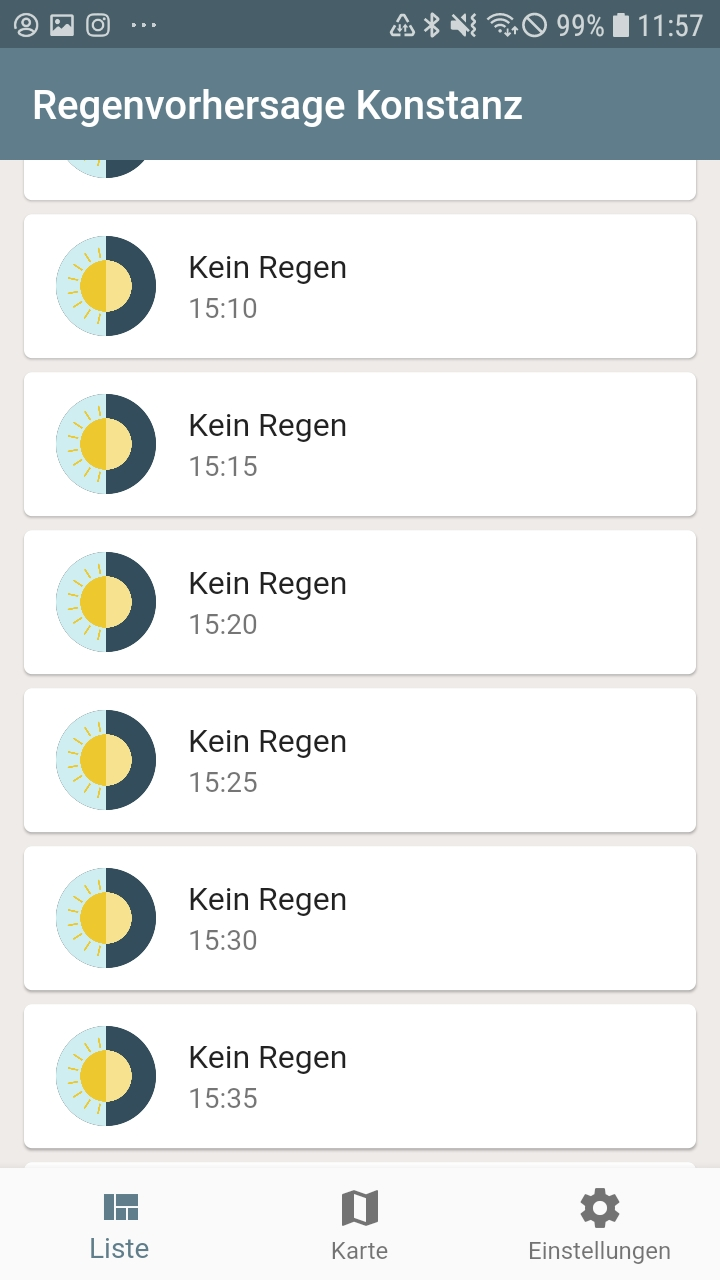
\includegraphics[width=0.3\linewidth]{abb/screenshot_forecast_list}}
    \subfloat[][]{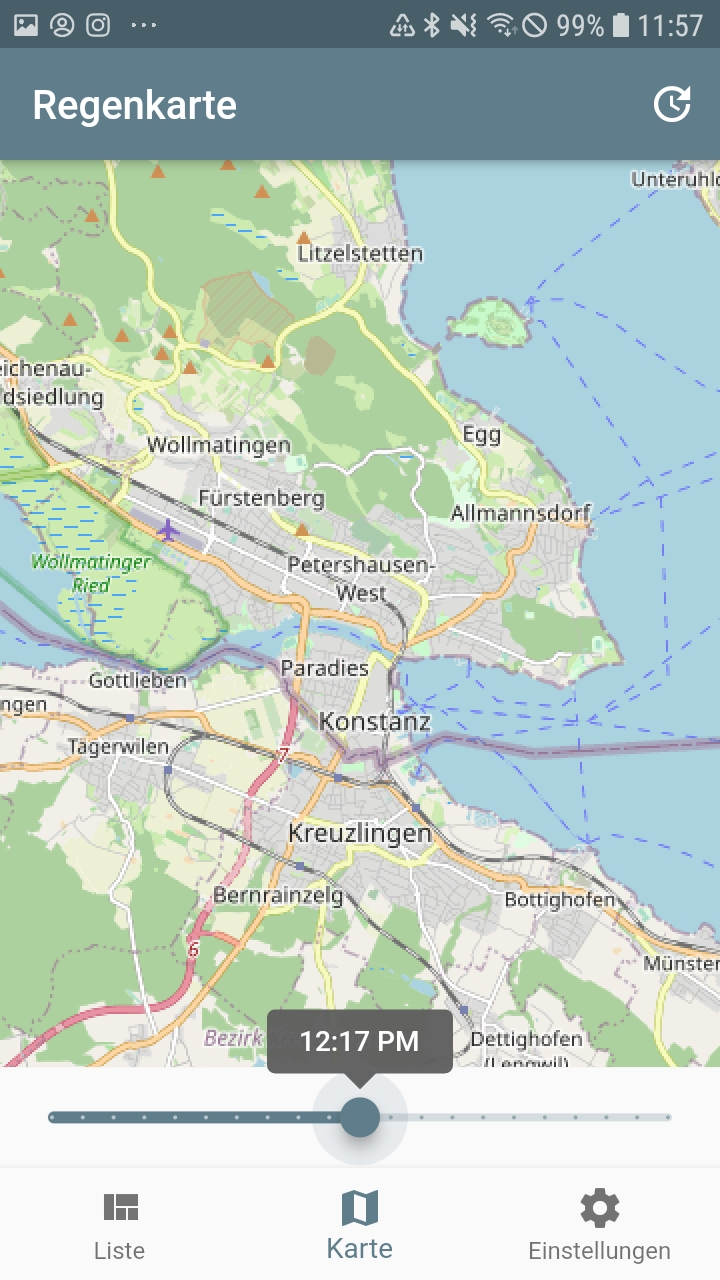
\includegraphics[width=0.3\linewidth]{abb/screenshot_forecast_map}}
    \subfloat[][]{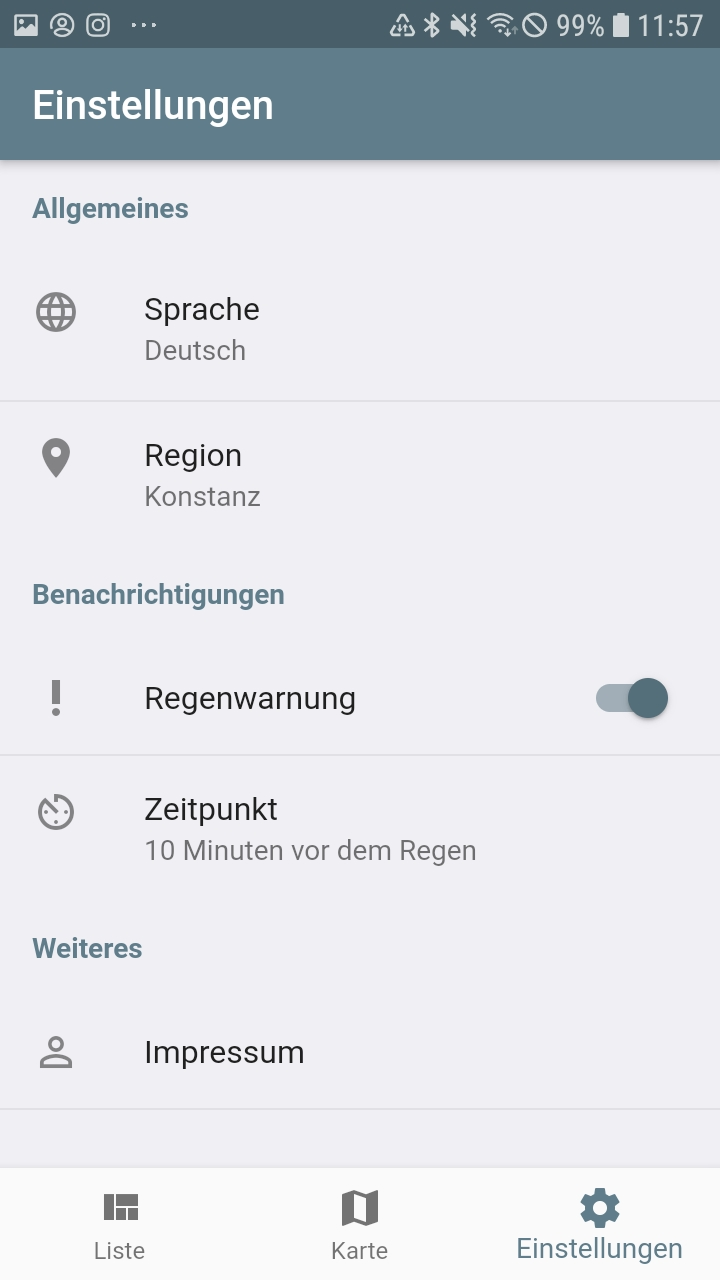
\includegraphics[width=0.3\linewidth]{abb/screenshot_settings}}
    \caption{Die drei Hauptscreens der App}
  \end{figure}

\subsubsection*{Regenvorhersage als Liste}
Auf diesem Screen werden die von den Netzen berechneten Regenvorhersagen angezeigt. 
Dabei wird in die drei Kategorien “Kein Regen”, “Leichter Regen” und “Starker Regen” unterschieden. 
Je höher die berechnete Regenintensität ist, je dunkler wird der Regenschirm welcher zu Beginn jedes einzelnen Listeneintrages zu sehen ist.   

\subsubsection*{Regenvorhersage als Karte}
Auf diesem Screen werden die von den Netzen erzeugten PNGs visualisiert. 
Dafür werden die PNGs mit einer Karte hinterlegt auf welcher der User frei navigieren kann, 
um die aktuelle Regensituation an jedem beliebigen Ort zu prüfen. 
Dabei wird standardmäßig der Kartenausschnitt von der Region angezeigt, die in den Einstellungen eingestellt wurde. 
Mit dem Slider kann der Zeitpunkt eingestellt werden, in dem die Regenvorhersage angezeigt werden soll. 
Mit dem Aktualisieren Button in der Actionbar können die neusten Bilder vom Server heruntergeladen werden. 
Im Normalfall werden die Bilder einmalig bei dem App Start heruntergeladen.  

\subsubsection*{Einstellungen}
Auf diesem Screen können alle relevanten Einstellungen gemacht werden. Dazu gehört z.B. die Sprache der Benutzeroberfläche. 
Außerdem kann die Region eingestellt werden. 
Die hier ausgewählte Region wird standardmäßig auf der Karte angezeigt und nur für diese Region werden Regenwarnungen gesendet. 
Unter der Benachrichtigung’s Kategorie können die Regenwarnungen Aktiviert werden sowie der Zeitpunkt der Regenwarnung eingestellt werden. 
Jede Aktion in dieser Kategorie löst eine Datenbankaktion aus. 
Wenn die Regenwarnung aktiviert wird, wird der Device Token von dem Gerät in die Datenbank hochgeladen, beim Deaktivieren wird der Device Token gelöscht. 
Wenn der Zeitpunkt der Regenwarnung verändert wird, wird der Device Token in der Datenbank von einer Kollektion in eine andere Kollektion verschoben.   
Alle gemachten Einstellungen werden in sogenannten Shared Preferences gespeichert, damit sie auch nach App Start immer noch vorhanden sind.   
In Abbildung \ref*{fig:sequence_diagram_change_settings} ist der Datenfluss beim anpassen des Zeitpunktes für die Regenwarnung 
nachvollzogen werden. 
In der folgenden Abbildung kann der Datenfluss nachdem der Zeitpunkt der Regenwarnung verändert wurde nachvollzogen werden.

\begin{figure}[H]
 \centering
 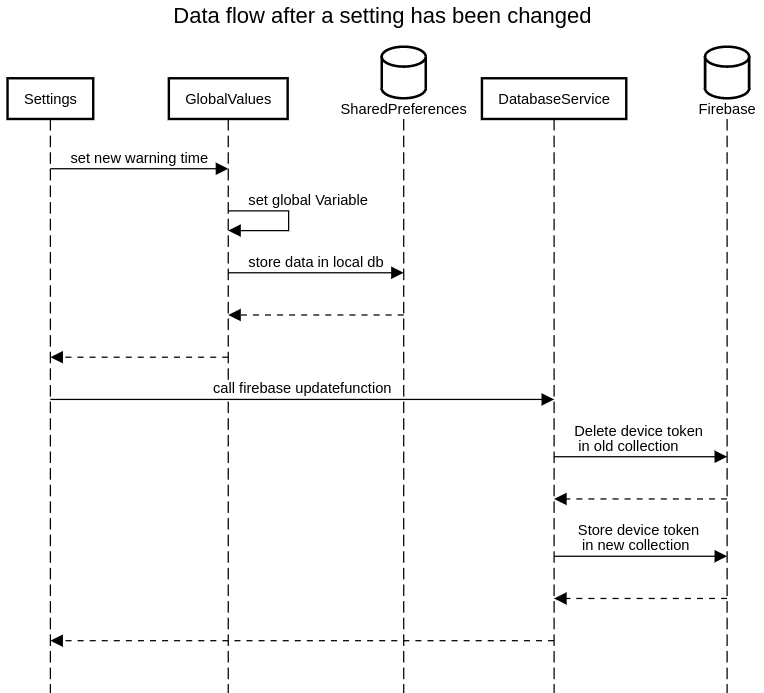
\includegraphics[width=0.8\textwidth,angle=0]{abb/sequence_diagram_change_settings}
 \caption[Sequencediagram Einstellungen ändern]{Der Datenfluss beim ändern des Zeitpunktes der Regenwarnung}
\label{fig:sequence_diagram_change_settings}
\end{figure}

\subsubsection{Der Appstart}
Während dem Appstart wird die App für die Verwendung vorbereitet, Einstellungen werden wieder hergestellt und
die aktuellen Regenvorhersagen werden aus der Datenbank heruntergeladen. 
Die Einstellungen können dabei aus den Shared Preferences ausgelesen werden. 
Die Shared Preferences sind eine lokale Key-Value Datenbank, in der alle benutzerspezifischen Daten gespeichert werden. 
Bei dem App Start werden die Einstellungen aus den Shared Preferences gelesen und auf globale Variablen gespeichert, somit
sind sie während der Laufzeit der App dynamisch verfügbar. 
Außerdem wird bei dem ersten Appstart die Position in dem Vorhersage Bild berechnet. 
Diese wird benötigt um aus den Vorhersage Bildern den richtigen Pixel auszulesen und in der Vorhersageliste anzuzeigen.
Der Appstart ist in folgender Abbildung schematisch dargestellt. 

\begin{figure}[H]
 \centering
 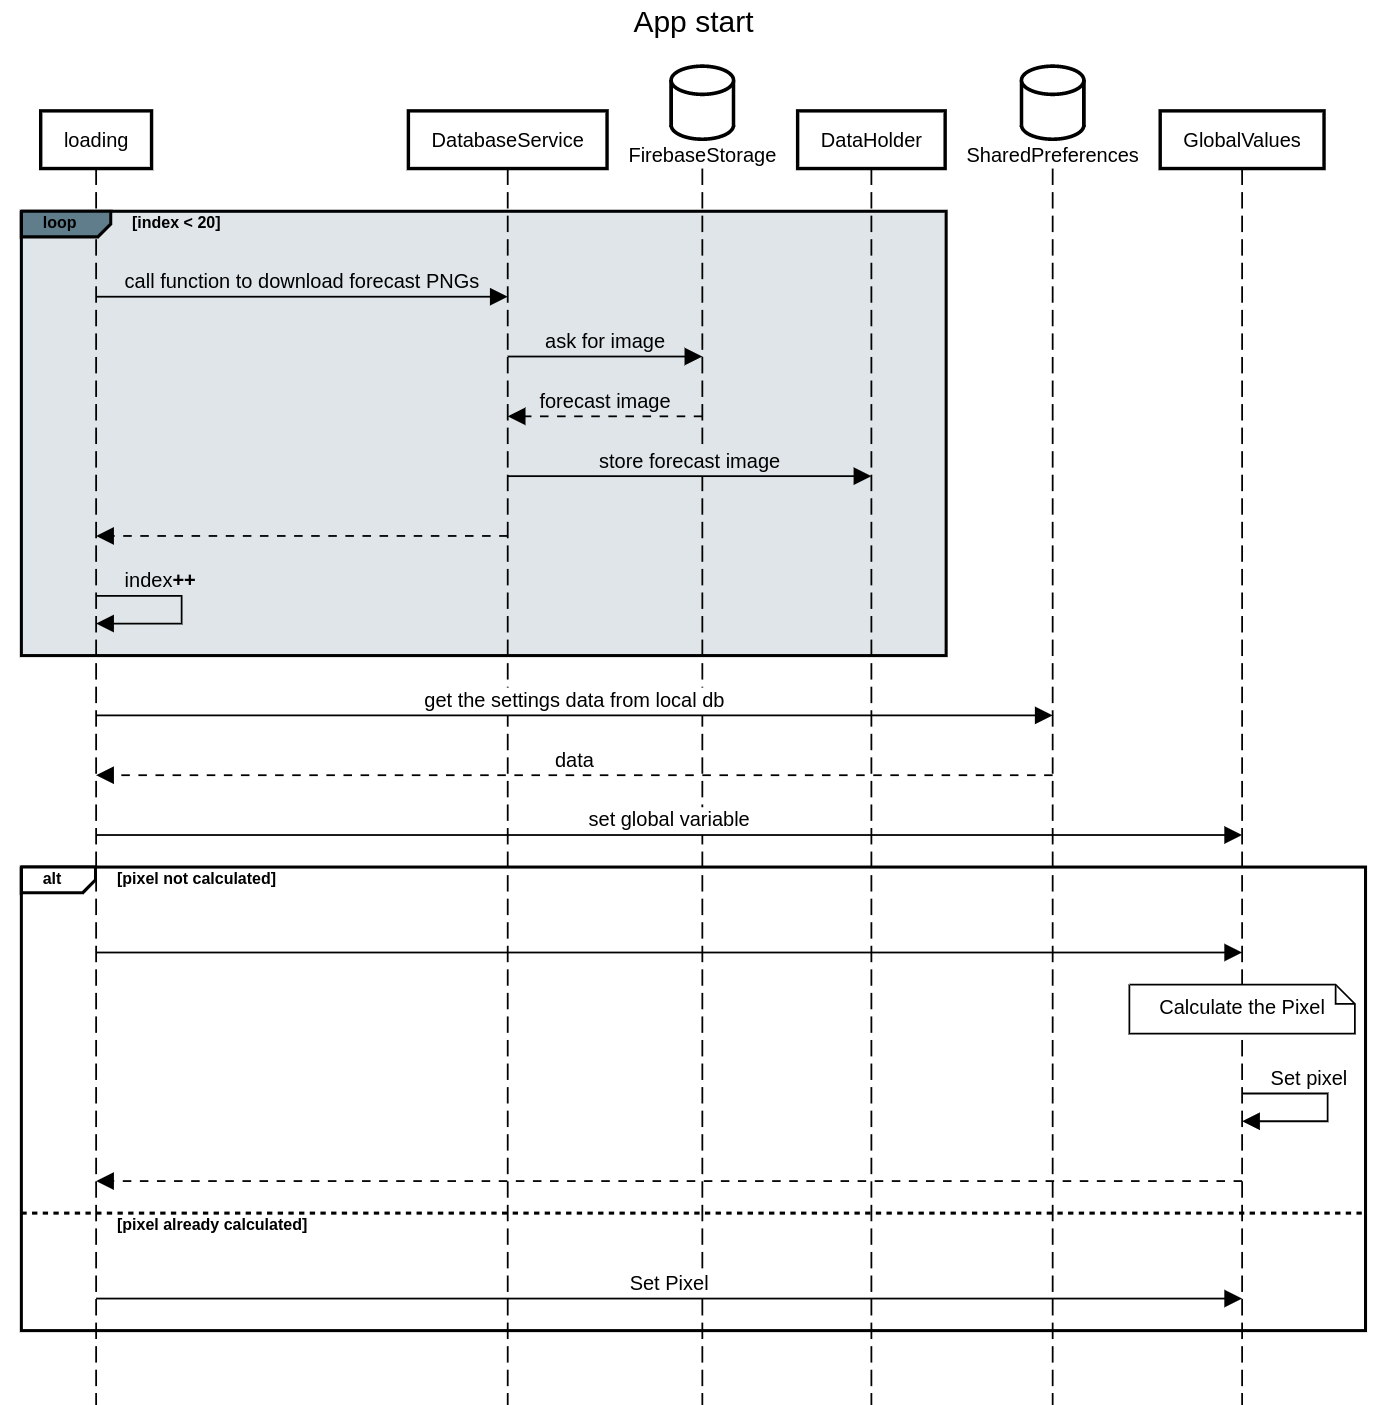
\includegraphics[width=0.8\textwidth,angle=0]{abb/sequence_diagram_app_start}
 \caption[Sequencediagram Appstart]{Datenfluss beim starten der App inklusive der Datenbankabfragen (Server und Lokale Datenbank)}
\label{fig:sequence_diagram_app_start}
\end{figure}

\subsubsection{Die Berechnung der Regenintensität}
Zu beginn wurde angenommen, dass die App nur in Konstanz verwendet werden soll. 
Im Laufe des Projektes stellte sich jedoch heraus, dass die entwickeleten Netze in der Lage sind, Vorhersagen 
für ganz Deutschland zu machen. Da die Software Architektur nicht für eine solche Anwendung ausgelegt war, 
mussten einige Änderungen vorgenommen werden. 
Bis zu diesem Zeitpunkt wurden die Vorhersage Daten für jeden Pixel auf dem Server berechnet und im Anschluss in 
der Firebase gespeichert. 
Bei verschiedenen Nutzern in verschiedenen Regionen kommt diese Architektur allerdings schnell an seine Grenzen. 
Hat die App bspw. 1000 Nutzer in verschiedenen Regionen, 
müssen für jeden der 1000 Nutzer, alle fünf Minuten, 20 Vorhersage Daten hochgeladen werden. 
Daher musste der Datenfluss so umstrukturiert werden, dass der neue Regenwert direkt in der App berechnet wird. 
Dabei muss das Handy den entsprechenden, eigenen, Pixel auf der Karte berechnen. 
Die Berechnung hierfür ist verhältnismäßig aufwändig, da mit großen Listen (810.000) Einträgen gearbeitet werden muss.
Auf diese Berechnung wird in Abschnitt \ref{sec: pixel_berechnung} eingegangen. 

Wenn die Bilder beim Appstart oder bei einem Vorhersageupdate heruntergeladen werden, wird von jedem Bild der Regenwert 
in dem entsprechnden Pixel berechnet. 
Es wird eine Liste mit ForecastListItem Objekten erstellt. Diese wird global gespeichert und in der Vorhersage Liste angezeigt. 
Aktuell können nur beim App Start und durch manuelles auslösen eines Updates die Vorhersage Daten aktualisiert werden.   

\subsubsection{Berechnung des Pixels} \label{sec: pixel_berechnung}
Um die Regensituation an dem jeweiligen Ort des Users auszuwerten, muss der Pixel in dem Vorhersagebild berechnet werden. 
Hierfür dienen drei verschiedene Listen. Diese Listen wurden in Python mit der Wradlib erstellt, und anschließend 
im JSON Format in die App übertragen. 
Zwei der Listen enthalten alle Latitude bzw. Longitude Werte.
Die Koordinaten in den einzelnen Indizes Kombiniert geben die Position der einzelnen Pixel im Weltkoordinatensystem an.
In der dritten Liste steht zu jedem Index die jeweilig zugehörige Pixel Koordinate im Bild. 
Somit steht jeder Index für eine Position im Weltkoordinatensystem, ausgedrückt durch Höhen und Breitengrad Informationen, 
und der Abbildung dieser Position auf den Vorhersagebild.
Da das Bild eine Auflösung von 900x900 Pixeln hat, sind diese Listen 810.000 Elemente groß. 
\begin{figure}[H]
  \centering
  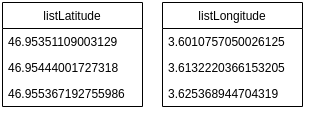
\includegraphics[width=0.8\textwidth,angle=0]{abb/listen_pixel_berechnung.png}
  \caption{Der Exemplarische Aufbau der Listen zur Berechnung des eigenen Pixels}
 \label{fig:sequence_diagram_app_start}
 \end{figure}
 Jeder User hat eine eigene Position in Deutschland, welche in Form von Höhen und Breitengrad angaben bekannt ist. 
 Diese wird durch die in den Einstellungen festgelegte Region bestimmt. 
 Es wird nun also ein Algorithmus gesucht, der mithilfe der Höhen und Breitengrad Informationen den Pixel im Bild findet, 
 der am besten zu diesen Koordinaten passt. 
 Nun wäre es natürlich möglich, durch alle Indizes zu Iterieren und somit den richtigen Pixel zu finden. Dieses Verfahren 
 ist aber sehr Zeit und Rechenintensiv und daher nicht geeignet um  es auf einem Smartphone auszuführen. 

 Wir brauchen noch eine Lösung!! 

\subsubsection{Framework Entscheidung}\label{framework entscheidung}
Bei der Entwicklung einer App steht die Frage der zu bedienenden Plattformen an erster Stelle. Soll die App zum Beispiel nur unternehmensintern verwendet 
werden oder ist das Gerät auf dem sie verwendet wird eine Neuanschaffung kann es ausreichend sein nativ auf einer Plattform zu entwickeln. Soll jedoch, 
wie bei den meisten Apps, eine breite Zielgruppe angesprochen werden, ist es unerlässlich die App auf IOS und Android zur Verfügung zu stellen. 
Je nach dem auf welchen Betriebssystemen die App verwendet werden soll, muss eine komplett andere Framework wahl getroffen werden. 
So würde man, wenn man entweder nur für IOS oder Android entwickeln möchte, zu einer der nativen Lösungen greifen. Je nach Anforderungen kann auch, 
wenn beide Betriebssysteme bedient werden sollen, zu der nativen Lösung gegriffen werden. In dem Fall muss der komplette Code natürlich doppelt 
geschrieben werden. Daher wird normalerweise auf Frameworks zurück gegriffen welche beide Betriebssysteme bedienen. 
Einige bekannte Frameworks sind zum Beispiel Xamarin, React Native oder Flutter. Jedes dieser Frameworks ist zukunftsträchtig und wurde von großen 
Unternehmen auf den Markt gebracht. So steht Microsoft hinter Xamarin, Facebook hinter React Native und Google hinter Flutter. 
Je nach Framework Wahl kann von ca. 80-100 Prozent von dem kompletten Code für beide Betriebssysteme verwendet werden. 
Dafür sind Cross-Plattform Frameworks oft nicht so performant wie die nativen. Dies fällt besonders bei rechenaufwändigen Apps und Spielen ins Gewicht. 
Bei so einer leichten App wie DeepRain fällt dieser Nachteil nicht ins Gewicht. Außerdem hätten wir auch nicht genug Kapazitäten um zwei native und 
voneinander unabhängige Apps zu entwickeln. 
Ein großer Vorteil von Flutter ist, dass 100 Prozent der Codebasis für Android und IOS übernommen werden können. Außerdem hat die Prominenz von 
Flutter in den letzten Jahren seit der Veröffentlichung stark zugenommen. In der folgenden Abbildung sind die Google Suchanfragen für den Begriff 
Flutter abgebildet.  Das in Kombination mit eigenem Interesse an dem Framework, ist der Grund dafür, dass die DeepRain App mit Flutter entwickelt wurde. 

\begin{figure}[h]
 \centering
 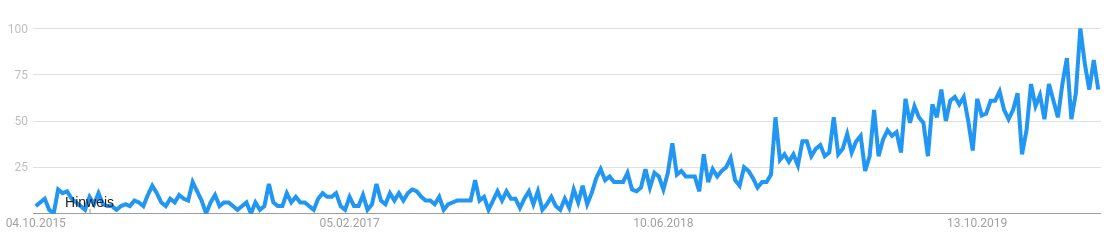
\includegraphics[width=0.8\textwidth,angle=0]{abb/flutter_google_trends}
 \caption[Entwicklung von Flutter]{Entwicklung der Suchanfragen für den Begriff 'Flutter'}
\label{fig:flutter_google_trends}
\end{figure}

\subsubsection{Technischer Aufbau von Flutter}
Flutter Anwendungen werden in der Programmiersprache Dart geschrieben und können anschließend für IOS, Android, Windows, Linux, MacOs und als WebApp 
veröffentlicht werden. Dart bringt dabei im Vergleich zu Java Script den Vorteil mit, dass es objektorientiert ist, was vor allem in größeren 
Softwarearchitekturen zum tragen kommt. Auch alle Bibliotheken um Code asynchron auszuführen werden bereits von Dart mitgeliefert. 
Die wohl größte Rolle für jeden Dart Entwickler spielen die sogenannten Widgets. Widgets sind einzelene Bausteine welche die UI repräsentieren. 
Jedes UI element ist dabei ein eigenes Widget. Dabei werden widgets oft ineinander geschachtelt, was es ermöglicht, komplexere UI’s zu entwerfen. 
Dabei werden Widgets in Stateless und Statefull Widgets unterschieden. Während ein Stateless Widget keine Daten und somit keinen Zustand speichern kann, 
ist das mit einem Stateful Widget möglich.

Die Grundlage von Flutter sind Widgets. \\
Wie funktioniert flutter?   \\
Was ist der Unterschied zu anderen hybriden Frameworks?  \\ 
Nur eine Codebasis \\
Keine weiteren Frameworks nötig\\
Alles dabei, UI, Widgets, Animationen\\

\subsubsection{Projektstruktur}
Der gesamte Code der App ist in die fünf Ordner DataObjects, global, screens, services und Widgets aufgeteilt. 
Die erste verwendete Datei ist main.dart. In dieser wird festgelegt welcher Screen als erstes nach dem Start 
aufgerufen wird und die Bottom Navigation wird konfiguriert. 
Für jeden Screen der App gibt es eine .dart datei in dem Ordner Screens. 
Welche Files gibt es? \\
Welche Klassen gibt es? \\
Wie arbeitet was zusammen? \\
\begin{figure}[H]
  \centering
  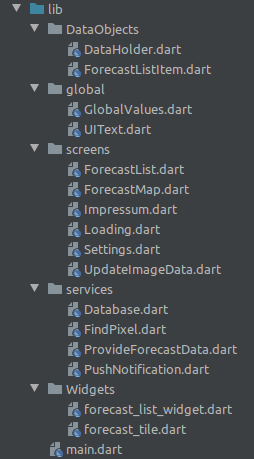
\includegraphics[width=0.3\textwidth,angle=0]{abb/projektstruktur}
  \caption{Die Projektstruktur der App}
 \label{fig:projektstruktur_app}
 \end{figure}

\subsection{Cloudfunktionen}
Mit den Cloud Funktionen von Firebase kann Backend-Code direkt auf den Servern von Google gespeichert und ausgeführt werden. 
Dabei ist es möglich, auf bestimmte Datenbank Aktionen zu reagieren. 
Diese Funktionalität wird verwendet, um Push Benachrichtigungen zu senden. 
Der Code wird in Java Script geschrieben und anschließend als Cloud Funktion hochgeladen. 

\subsubsection{Push Benachrichtigungen}\label{sec:Pushbenachrichtigungen}
Zum Warnen der Benutzer, wenn es eine Regenvorhersage gibt, werden Push Nachrichten verwendet. 
Der Zeitpunkt der Push Benachrichtigungen kann in der App eingestellt werden. 
So kann man sich zwischen 5 und 60 Minuten vor dem bevorstehenden Regen warnen lassen.  
Um eine Push Benachrichtigung zu versenden speichert der Server ein Dokument in der Firebase welches alle für die 
Push Benachrichtigung relevanten Informationen enthält. 
Dazu gehört zum Beispiel der Push Benachrichtigungs Titel und Text, sowie die Zeit bis der Regen eintritt.
Sobald das neue Dokument mit den Informationen für die Push Benachrichtigung hochgeladen wurde, wird eine Callback 
Funktion in form einer Cloudfunktion aufgerufen.
Je nach dem zu welchem Zeitpunkt ein User die Regenwarnung erhalten möchte, wird sein Device Token in eine andere 
Kollektion gespeichert.   
Außerdem wird je nach Region in der sich der User befindet, sein Token in einer anderen Kollektion gespeichert. 
Nur die Tokens, die sowohl mit dem Zeitpunkt, als auch mit der Region, aus dem vom Server hochgeladenen Dokument übereinstimmen, 
sollen eine Push Benachrichtigung erhalten. 
Die Funktion findet diese Schnittmenge und weiß somit, welche Geräte eine Pushbenachrichtigung erhalten sollen. 

\begin{figure}[h]
 \centering
 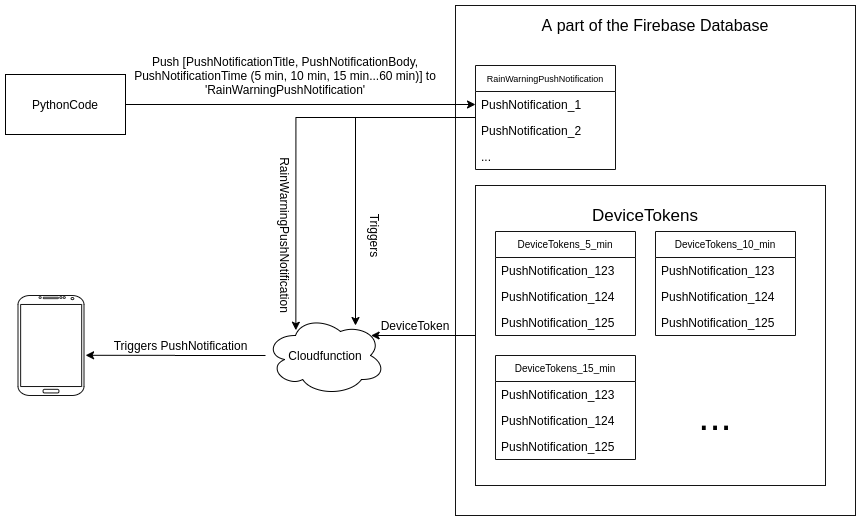
\includegraphics[width=0.8\textwidth,angle=0]{abb/funktionsweise_pushnachrichten_senden}
 \caption[Funktionsweise von Pushbenachrichtigungen]{Funktionsweise des Prozesses zum senden von Push - Benachrichtigungen.}
\label{fig:funktionsweise_pushnachrichten_senden}
\end{figure}

\subsection{Vorgehen bei Entwicklung}
In Flutter entwickelte Apps können sowohl auf Android als auch auf IOS ausgeführt werden. 
Um eine Flutter App auf einem IPhone auszuführen, wird allerdings MacOS als Betriebssystem benötigt. 
Da während des Entwicklungsprozesses nur ein Linux Rechner zur Verfügung stand, wurde die App lange Zeit nur unter
Android getestet. 
Erst gegen ende des Projektes wurde der Code für IOS kompiliert und für das IPhone angepasst.  
Da die gesamte Pipeline zu beginn noch nicht funktioniert hat, wurde der für die App relevante Teil der Pipeline simuliert.
Dazu wurde ein Python Programm geschrieben, welches reale Daten in die Firebase pushed. 
Somit war es möglich, gekapselt vom rest des Projektes zu arbeiten, und die App fertig zu stellen. 
 


    

